\section{Discussion of physics implications}
\label{sec:discussion}

One very comprehensive (and therefore representative) studies of the pre-LHC data is by the COMPETE collaboration \cite{compete}. In total 256 models were been considered to describe $\sigma_{\rm tot}$ and $\rho$ data for various reactions ($\rm pp$, $\rm p\pi$, $\rm pK$, etc.) and the related reactions with antiparticles. Out of these models, 23 have been found to give a reasonable description of the data \cite{compete-details}. Extrapolations from these models are confronted with newer TOTEM measurements in Figure~\ref{fig:comp bands}, which shows that they are grouped 3 bands. Each band is plotted in a different colour and has a different level of compatibility with the data. As argued above, the $13\un{TeV}$ fit with $N_b=1$ and $|t|_{\rm max} = 0.07\un{GeV^2}$ (rightmost point in the figure) corresponds to the most fair comparison to past analyses and is therefore used to evaluate the compatibility with the COMPETE models. The $8\un{TeV}$ $\rho$ point is not included in this calculation since it does not bring any information due to its large uncertainty. The $\sigma_{\rm tot}$ measurements can be, to a large extent, regarded as independent: they used data from different LHC fills at different energies, different beam optics, often different RPs, often different analysis approaches (fit parametrisation, treatment of CNI) and often they were analysed by different teams. The only correlation comes from using common normalisation at a given collision energy. Consequently, two compatibility evaluations were made: using all $\sigma_{\rm tot}$ points from Figure~\ref{fig:comp bands} and using their subset with a single point per energy. These two results thus provide upper and lower bounds for the actual compatibility level. The observations can be summarised as follows.
\begin{itemize}[noitemsep,topsep=0pt]
\item The blue band is compatible (p-value $0.990$ to $0.995$) with the $\sigma_{\rm tot}$ data, but incompatible (p-value $1\times10^{-6}$) with the $\rho$ point.
\item The magenta band is incompatible (p-value $4\times10^{-4}$ to $4\times10^{-6}$) with the $\sigma_{\rm tot}$ data and incompatible (p-value $5\times10^{-3}$) with the $\rho$ point.
\item The green band is incompatible (p-value $3\times10^{-9}$ to $2\times10^{-19}$) with the $\sigma_{\rm tot}$ data, but compatible (p-value $0.32$) with the $\rho$ point.
\end{itemize}
In summary, none of the COMPETE models is compatible with the ensemble of TOTEM's $\sigma_{\rm tot}$ and $\rho$ measurements.

\begin{figure*}
\vskip-5mm
\begin{center}
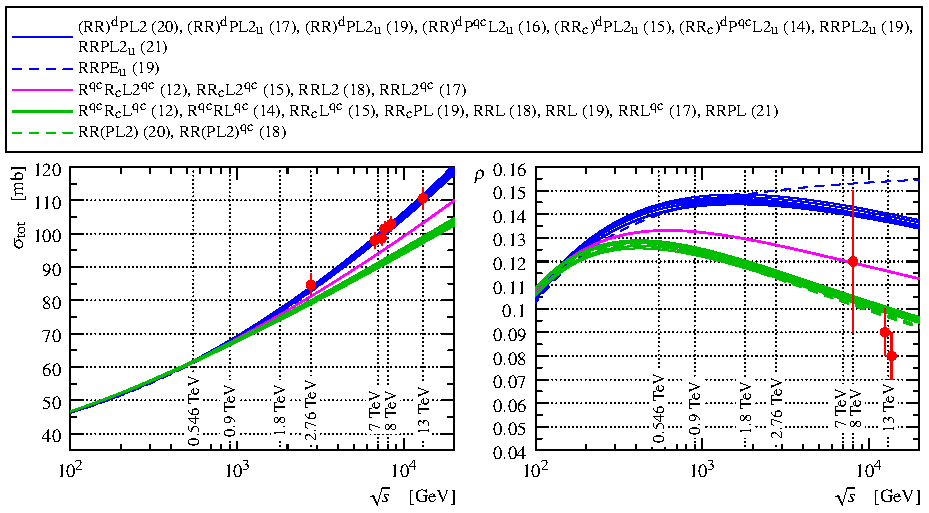
\includegraphics{fig/compete_bands_si_tot_rho.pdf}
\caption{%
Predictions of COMPETE models \cite{compete-details} for $\rm pp$ interactions. Each model is represented by one line (see legend). The red points represent the reference TOTEM measurements. The two $\rho$ points at $13\un{TeV}$ correspond to the two cases discussed in Section~\ref{sec:rho anal}: the left point to the fit with $N_b=3$ and $|t|_{\rm max} = 0.15\un{GeV^2}$, the right point to $N_b=1$ and $|t|_{\rm max} = 0.07\un{GeV^2}$.
}
\label{fig:comp bands}
\end{center}
\end{figure*}

Another, even less model-dependent, relation between $\sigma_{\rm tot}$ and $\rho$ can be obtained from dispersion relations \TODO{reference}. If only the crossing-even component of the amplitude is considered, it can be shown that $\rho$ is proportional to the rate of growth of $\sigma_{\rm tot}$ with energy. This is in contradiction to the presented data featuring sustained growth of $\sigma_{\rm tot}$ while a low value of $\rho$.

The above observations seem to suggest a need for an odd-signature object being exchanged by the protons. While at lower energies such contributions may naturally come from secondary Reggeons \TODO{examples}, the contribution of the latter is generally considered negligible at LHC energies due to their intercept lower than unity.

A variety of such odd-signature exchange contributions have been discussed in literature, within different frameworks and under different names. The ``Odderon'' was introduced within the axiomatic theory \cite{nicolescu-1990,nicolescu-2007} as an amplitude contribution responsible for $\sigma_{\rm tot}^{\rm p\bar p} - \sigma_{\rm tot}^{\rm pp} \propto \log s$ and also for the $\rm p\bar p$ and $\rm pp$ difference of the differential cross-section in the dip region. Crossing-even trajectories were also studied within the framework of Regge theory as a counterpart of the crossing-even Pomeron \TODO{reference}. It has also been shown that an such object must exist in QCD, as a colourless bound state of three gluons with quantum numbers $J^{PC} = 1^{--}$ \TODO{reference}. These 3 gluons are bound together more strongly than their interaction with other particles is. There is also evidence for such a state in QCD lattice calculations, known under the names ``oddball'' or ``vector glueball'' \TODO{reference}. Such a state can be exchanged in the $t$-channel and contribute, e.g., to the elastic-scattering amplitude, as well as can be created in the $s$-channel and thus be observed in spectroscopic studies. More details can be found in reviews \cite{braun,ewerz}.

There are multiple ways how an odd-signature exchange component may manifest in observable data. Focusing on elastic scattering at the LHC (unpolarised beams), there are 3 regions argued to be sensitive. In general, the effects of an odd-signature exchange (3 bound gluons) are expected to be much smaller compared to those of even-signature exchanges (2 bound gluons). Consequently, the sensitive regions are those where the contributions from 2-bound-gluon exchanges cancel or are limited in size. At very low $|t|$ the 2-bound-gluon amplitude is expected to be almost purely imaginary, while a 3-gluon exchange would make contributions to the real part and therefore $\rho$ is a very sensitive parameter. Another such example is the dip, often described as the imaginary part of the amplitude crossing zero, thus ceding the dominance to the real part to which a 3-gluon exchange may contribute. In agreement with such predictions, the observed dips in $\rm p\bar p$ scattering are shallower than those in $\rm pp$. At $\sqrt s \approx 62\un{GeV}$, there are data showing a very significant difference between the $\rm pp$ and $\rm p\bar p$ dip. The interpretation of this difference is, however, complicated due to non-negligible contribution from secondary Reggeons. This dip difference is also predicted to be energy-dependent which presents another experimental observable. Sometimes high $|t|$ region is also argued to be sensitive to 3-gluon exchanges since the contribution from 2-gluon exchanges is rapidly dropping. However, preliminary high-$|t|$ TOTEM data at $13\un{TeV}$ indicate that this region is dominated by yet another perturbative-QCD amplitude \TODO{ref to Landshoff}.

\begin{figure*}
\vskip-5mm
\begin{center}
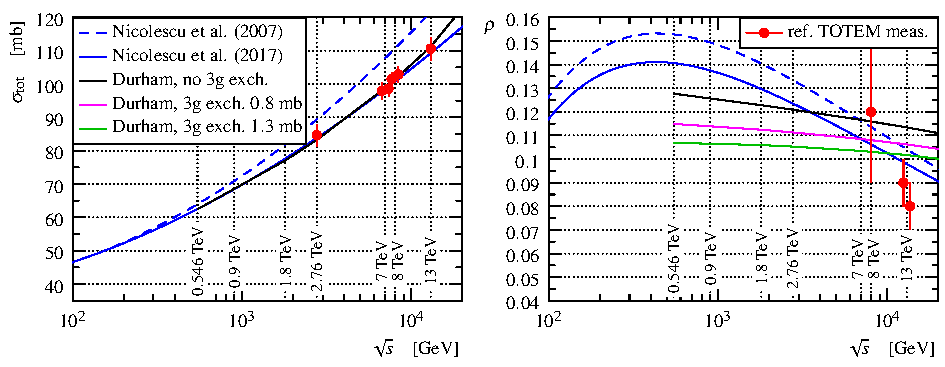
\includegraphics{fig/matching_models_si_tot_rho.pdf}
\caption{%
Predictions of the model by Nicolescu et al.~\cite{nicolescu-2017} (blue) and the Durham model \cite{durham-2017-note} (green) compared to the reference TOTEM measurements (red). For the Durham model the dashed (solid) curve corresponds to the prediction with (without) odd-signature exchange component. The two $\rho$ points at $13\un{TeV}$ correspond to the two cases discussed in Section~\ref{sec:rho anal}: the left point to the fit with $N_b=3$ and $|t|_{\rm max} = 0.15\un{GeV^2}$, the right point to $N_b=1$ and $|t|_{\rm max} = 0.07\un{GeV^2}$.
}
\label{fig:match models}
\end{center}
\end{figure*}

Figure~\ref{fig:match models} compares the TOTEM data with two compatible models: by Nicolescu et al.~\cite{nicolescu-2017} and the Durham model \cite{durham-2017-note}. In both cases, inclusion of a crossing-odd exchange component leads to an improvement of the agreement between the data and model. For the Nicolescu model, the effect is almost negligible at $\sqrt s \approx 500\un{GeV}$ but its size grows with energy making it very significant at $13\un{TeV}$. Conversely, in the Durham model the effect is sizeable at $\sqrt s \approx 500\un{GeV}$ and gently diminishes with energy. The energy dependence of $\rho$ is predicted to be rather flat unlike the strong energy dependence in the Nicolescu model. Therefore, precise $\rho$ measurements at $\sqrt s \approx 900\un{GeV}$ and $14\un{TeV}$ would be valuable for discrimination between these models.
